\documentclass[11pt]{article}
\usepackage[a4paper,margin=2.25cm]{geometry}
\usepackage{amsmath,amssymb,bm}
\usepackage{graphicx}
\usepackage{booktabs}
\usepackage{tabularx}
\usepackage{xcolor}
\usepackage{float}
\usepackage[font=small,labelfont=bf]{caption}
\usepackage{hyperref}
\hypersetup{colorlinks=true,linkcolor=blue!45!black,citecolor=blue!45!black,urlcolor=blue!55!black}
\setlength{\parskip}{0.35em}
\setlength{\parindent}{0pt}
\newcommand{\SO}{\mathrm{SO}}
\newcommand{\ks}{\mathbf{k}s}
\newcommand{\psim}{|\Psi^-\rangle}

\title{\textbf{Applicability of the Oh--Kim two-spin density matrix\\to the Hubbard--Rashba BdG model}\\[0.5em]
\large Scientific assessment of Eq.~(19) of Oh and Kim for the model of Hutchinson, Hirsch, and Marsiglio}
\author{Reproducible analysis of the repository calculation}
\date{7 November 2026}

\begin{document}
\maketitle

\begin{abstract}
\noindent
The Oh--Kim two-spin density matrix is applicable to the archived zero-spin-orbit-coupling calculation, but translational invariance alone is not a sufficient justification. The required assumptions are a spatially uniform lattice state, pairing at zero center-of-mass momentum, a Gaussian BdG mean-field state, a spin-diagonal normal correlator, a spin-singlet anomalous correlator, and normalization conditional on detecting one electron at each of two positions. The uniform Hutchinson--Hirsch--Marsiglio Hamiltonian and its zero-momentum BdG mean field satisfy the first three assumptions. At $V_{\SO}=0$, the original spin basis also satisfies the spin-diagonal and singlet assumptions. Momentum dependence or a sign change of the extended-$s$-wave gap, and direction dependence on a square lattice, do not break translational invariance. The same matrix cannot be applied without generalization to physical spin qubits at nonzero Rashba coupling, where the base model contains mixed singlet--triplet pairing and spin-off-diagonal normal correlations. A separate numerical issue remains in the archived anomalous input: non-negative coherence amplitudes discard the sign of $\Delta_{\mathbf k}$ before Brillouin-zone integration. This input issue does not invalidate the Oh--Kim matrix algebra.
\end{abstract}

\textbf{Repository state analyzed:} \texttt{dc7f25fc3757077a2a764fadbd726f27da4b6d4d}.\\
\textbf{Archived numerical case:} $U/t=75$, $\Delta_t/t=4.5$, $V_{\SO}=0$, $n=1.875$, $N_k=100$, $T=0$.

\section{Conclusion}

The defensible conclusion is:
\begin{quote}
The Oh--Kim reduction is used only for the spatially uniform, zero-center-of-mass-momentum BdG mean-field state at $V_{\SO}=0$. In that limit the normal Green function is spin diagonal and the anomalous Green function is an even-parity spin singlet. Together with Wick factorization and conditional two-electron normalization, these assumptions yield Oh--Kim Eqs.~(19)--(23), including for a momentum-dependent extended-$s$-wave gap. The same expression is not claimed for original-spin qubits at nonzero Rashba coupling.
\end{quote}

Thus, the matrix can be used for the present archived $V_{\SO}=0$ model, subject to the anomalous-coherence correction in Sec.~\ref{sec:signed}. It is not sufficient to defend it solely by saying that the Hamiltonian is translational invariant.

\section{Assumptions in the Oh--Kim derivation}

Oh and Kim derive the two-electron density matrix from a two-particle Green function~\cite{OhKim}. Their derivation requires:
\begin{enumerate}
    \item \textbf{Gaussian BCS state.} Their Eq.~(7) factorizes the two-particle Green function by Wick's theorem. This is a BCS/BdG mean-field property, not an identity for an arbitrary exact interacting Hubbard state.
    \item \textbf{Spin-diagonal normal propagation.} Their Eqs.~(8a)--(8b) use $G_{ss'}(\mathbf r,\mathbf r')\propto\delta_{ss'}G(\mathbf r-\mathbf r')$.
    \item \textbf{Singlet anomalous propagation.} Their Eqs.~(9a)--(9c) use the antisymmetric spin structure $I_{ss'}=i\sigma_y$.
    \item \textbf{Translational invariance.} Their discussion before Eqs.~(10)--(13) uses $G(\mathbf r_1,\mathbf r_1')=G(\mathbf r_1-\mathbf r_1')$ and $F(\mathbf r_1,\mathbf r_2)=F(\mathbf r_1-\mathbf r_2)$.
    \item \textbf{Diagonal spatial detection.} Their Eq.~(19) sets $\mathbf r_1=\mathbf r_1'$ and $\mathbf r_2=\mathbf r_2'$, describing one electron detected at each of two locations.
    \item \textbf{Conditional normalization.} Their Eqs.~(20)--(21) normalize the resulting two-electron detection sector to a two-spin state.
\end{enumerate}

\section{Proof of translational invariance for the base model}

\subsection{Uniform lattice Hamiltonian}

Let $T_{\mathbf a}$ translate every lattice site by a lattice vector $\mathbf a$:
\begin{equation}
T_{\mathbf a}c_{i\sigma}T_{\mathbf a}^{-1}=c_{i+\mathbf a,\sigma}.
\end{equation}
The normal hopping in Hutchinson \emph{et al.}~\cite{Hutchinson} is a sum over identical nearest-neighbor bonds, the Hubbard interaction has site-independent $U$, and the correlated-hopping coefficient $\Delta t$ is site independent. Their Rashba term has the same oriented bond structure at every site. Therefore, for an infinite lattice or periodic boundary conditions,
\begin{equation}
T_{\mathbf a}HT_{\mathbf a}^{-1}=H.
\end{equation}
Rashba coupling can break inversion or spin-rotation symmetry without breaking discrete lattice translations.

\subsection{Zero-momentum pairing}

The retained mean-field pairs have the form $c_{\mathbf k\alpha}^{\dagger}c_{-\mathbf k\beta}^{\dagger}$, with zero total momentum. Using
\begin{equation}
c_{j\sigma}=\frac1{\sqrt N}\sum_{\mathbf k}e^{i\mathbf k\cdot\mathbf R_j}c_{\mathbf k\sigma},
\end{equation}
the normal equal-time correlator becomes
\begin{align}
\langle c_{i\sigma}^{\dagger}c_{j\sigma}\rangle
&=\frac1N\sum_{\mathbf k,\mathbf k'}e^{-i\mathbf k\cdot\mathbf R_i+i\mathbf k'\cdot\mathbf R_j}
\langle c_{\mathbf k\sigma}^{\dagger}c_{\mathbf k'\sigma}\rangle\notag\\
&=\frac1N\sum_{\mathbf k}e^{i\mathbf k\cdot(\mathbf R_j-\mathbf R_i)}n_{\mathbf k\sigma}
=G_\sigma(\mathbf R_j-\mathbf R_i).
\end{align}
Similarly,
\begin{equation}
\langle c_{i\uparrow}c_{j\downarrow}\rangle
=\frac1N\sum_{\mathbf k}e^{i\mathbf k\cdot(\mathbf R_i-\mathbf R_j)}
\langle c_{\mathbf k\uparrow}c_{-\mathbf k\downarrow}\rangle
=F_{\uparrow\downarrow}(\mathbf R_i-\mathbf R_j).
\end{equation}
A simultaneous translation of $\mathbf R_i$ and $\mathbf R_j$ leaves both expressions unchanged.

\subsection{Momentum-dependent and sign-changing gaps are allowed}

Nothing in this proof requires $\Delta_{\mathbf k}$ to be constant or positive. The gap
\begin{equation}
\Delta_{\mathbf ks}=\Delta_0-\frac{\Delta_s}{4t}\epsilon_{\mathbf ks}
\end{equation}
depends on relative crystal momentum; it is not a position-dependent potential or a finite-momentum pair field. Its sign changes modify $F(\mathbf r)$ but do not invalidate $F(\mathbf R_1,\mathbf R_2)=F(\mathbf R_1-\mathbf R_2)$.

A square lattice need not be continuously rotationally invariant. Thus $G$ and $F$ may depend on the direction of $\mathbf r$. Oh--Kim Eq.~(19) can be read with vector separation; continuous rotational symmetry is not required for the spin algebra.

Open boundaries, impurities, position-dependent mean fields, finite-momentum pairing, or spontaneous translational symmetry breaking would require two-position correlators. A finite Brillouin-zone quadrature grid is not, by itself, an open-boundary real-space model.

\section{From Wick factorization to the Oh--Kim matrix}

For a quadratic BdG Hamiltonian, the equal-time contraction has the generic structure
\begin{align}
\langle c_{2'}^{\dagger}c_{1'}^{\dagger}c_1c_2\rangle
={}&\langle c_{2'}^{\dagger}c_2\rangle\langle c_{1'}^{\dagger}c_1\rangle
-\langle c_{2'}^{\dagger}c_1\rangle\langle c_{1'}^{\dagger}c_2\rangle\notag\\
&+\langle c_{2'}^{\dagger}c_{1'}^{\dagger}\rangle\langle c_1c_2\rangle .
\end{align}
At two detected positions, translational invariance reduces the normal factors to $G(0)$, $G(\mathbf r)$, and $G(-\mathbf r)$, while the anomalous factor contains $F(\mathbf r)F^*(\mathbf r)$. With the spin structures above, this is Oh--Kim Eq.~(19).

Define
\begin{equation}
g(\mathbf r)=\frac{G(\mathbf r)}{G(0)},\qquad
f(\mathbf r)=\frac{F(\mathbf r)}{G(0)},
\end{equation}
and write $g^2=|g(\mathbf r)|^2$, $f^2=|f(\mathbf r)|^2$. Conditional normalization gives
\begin{equation}
\rho_X(\mathbf r)=\frac1{\mathcal N}
\begin{pmatrix}
1-g^2&0&0&0\\
0&1+f^2&-(g^2+f^2)&0\\
0&-(g^2+f^2)&1+f^2&0\\
0&0&0&1-g^2
\end{pmatrix},
\qquad \mathcal N=4-2g^2+2f^2.
\label{eq:X}
\end{equation}
The microscopic momentum dependence enters through $g$ and $f$; it does not change this spin algebra.

\section{Algebraic proof of Werner form and positivity}

Define
\begin{equation}
p=\frac{f^2+g^2}{2+f^2-g^2},\qquad
|\Psi^-\rangle=\frac{|\uparrow\downarrow\rangle-|\downarrow\uparrow\rangle}{\sqrt2}.
\end{equation}
Direct expansion proves
\begin{equation}
\rho_X=(1-p)\frac{\mathbb I_4}{4}+p|\Psi^-\rangle\langle\Psi^-|.
\label{eq:W}
\end{equation}
The eigenvalues are
\begin{equation}
\lambda_s=\frac{1+3p}{4},\qquad \lambda_t=\frac{1-p}{4}\quad\text{(threefold)},
\end{equation}
or, equivalently,
\begin{equation}
\lambda_t=\frac{1-g^2}{\mathcal N},\qquad
\lambda_s=\frac{1+g^2+2f^2}{\mathcal N}.
\end{equation}
Because $G(\mathbf r)$ is a normalized weighted sum of phases,
\begin{equation}
|g(\mathbf r)|=\left|\frac{\sum_{\mathbf k}w_{\mathbf k}e^{i\mathbf k\cdot\mathbf r}}
{\sum_{\mathbf k}w_{\mathbf k}}\right|\leq1,\qquad w_{\mathbf k}\geq0.
\end{equation}
Hence $g^2\leq1$, $\mathcal N\geq2+2f^2>0$, $\lambda_t\geq0$, and $0\leq p\leq1$. The conditional matrix is Hermitian, unit trace, and positive semidefinite. At $\mathbf r=0$, $g=1$, so $p=1$ and $\rho_X(0)=|\Psi^-\rangle\langle\Psi^-|$ independently of $f(0)$.

These results prove consistency of the matrix form; they do not independently prove that a particular numerical implementation has calculated $G$ and $F$ correctly.

\section{Application to the archived model}

\begin{table}[H]
\centering
\small
\begin{tabularx}{\textwidth}{p{0.29\textwidth}p{0.38\textwidth}X}
\toprule
Requirement & Assessment & Evidence \\
\midrule
Uniform square lattice & Satisfied for the stated infinite/periodic bulk model & Base Hamiltonian; \texttt{kspace\_setup.py} \\
Zero total pair momentum & Satisfied & Hutchinson \emph{et al.} Eqs.~(14), (19)--(22) \\
Gaussian Wick factorization & Satisfied within BdG mean field, not an exact non-Gaussian Hubbard treatment & Mean-field decoupling in base paper \\
Spin-diagonal normal correlator & Satisfied at $V_{\SO}=0$ & \texttt{config.py}; degenerate helicity branches \\
Singlet anomalous spin structure & Satisfied at $V_{\SO}=0$ for even extended-$s$-wave pairing & Original spin basis restored \\
Relative-coordinate correlators & Satisfied by the Fourier construction & \texttt{greens\_functions.py}; translation proof \\
Conditional two-location state & Matches the intended construction & \texttt{density\_matrix.py} implements Eqs.~(20)--(21) \\
Original-spin use at nonzero Rashba coupling & \textbf{Not valid without generalization} & Sec.~\ref{sec:rashba} \\
Exact signed anomalous input & \textbf{Not satisfied by archived unsigned amplitudes when the gap changes sign} & Sec.~\ref{sec:signed} \\
\bottomrule
\end{tabularx}
\caption{Assumption-by-assessment summary. Source-code checks and analytical derivations are distinguished from the numerical tests below.}
\end{table}

Hutchinson \emph{et al.} explicitly state that their Rashba gap is mixed singlet--triplet; see their Eq.~(31) and surrounding discussion~\cite{Hutchinson}.

\section{Numerical checks and figures}

\subsection{Spatial correlators and lattice symmetry}

\begin{figure}[H]
\centering
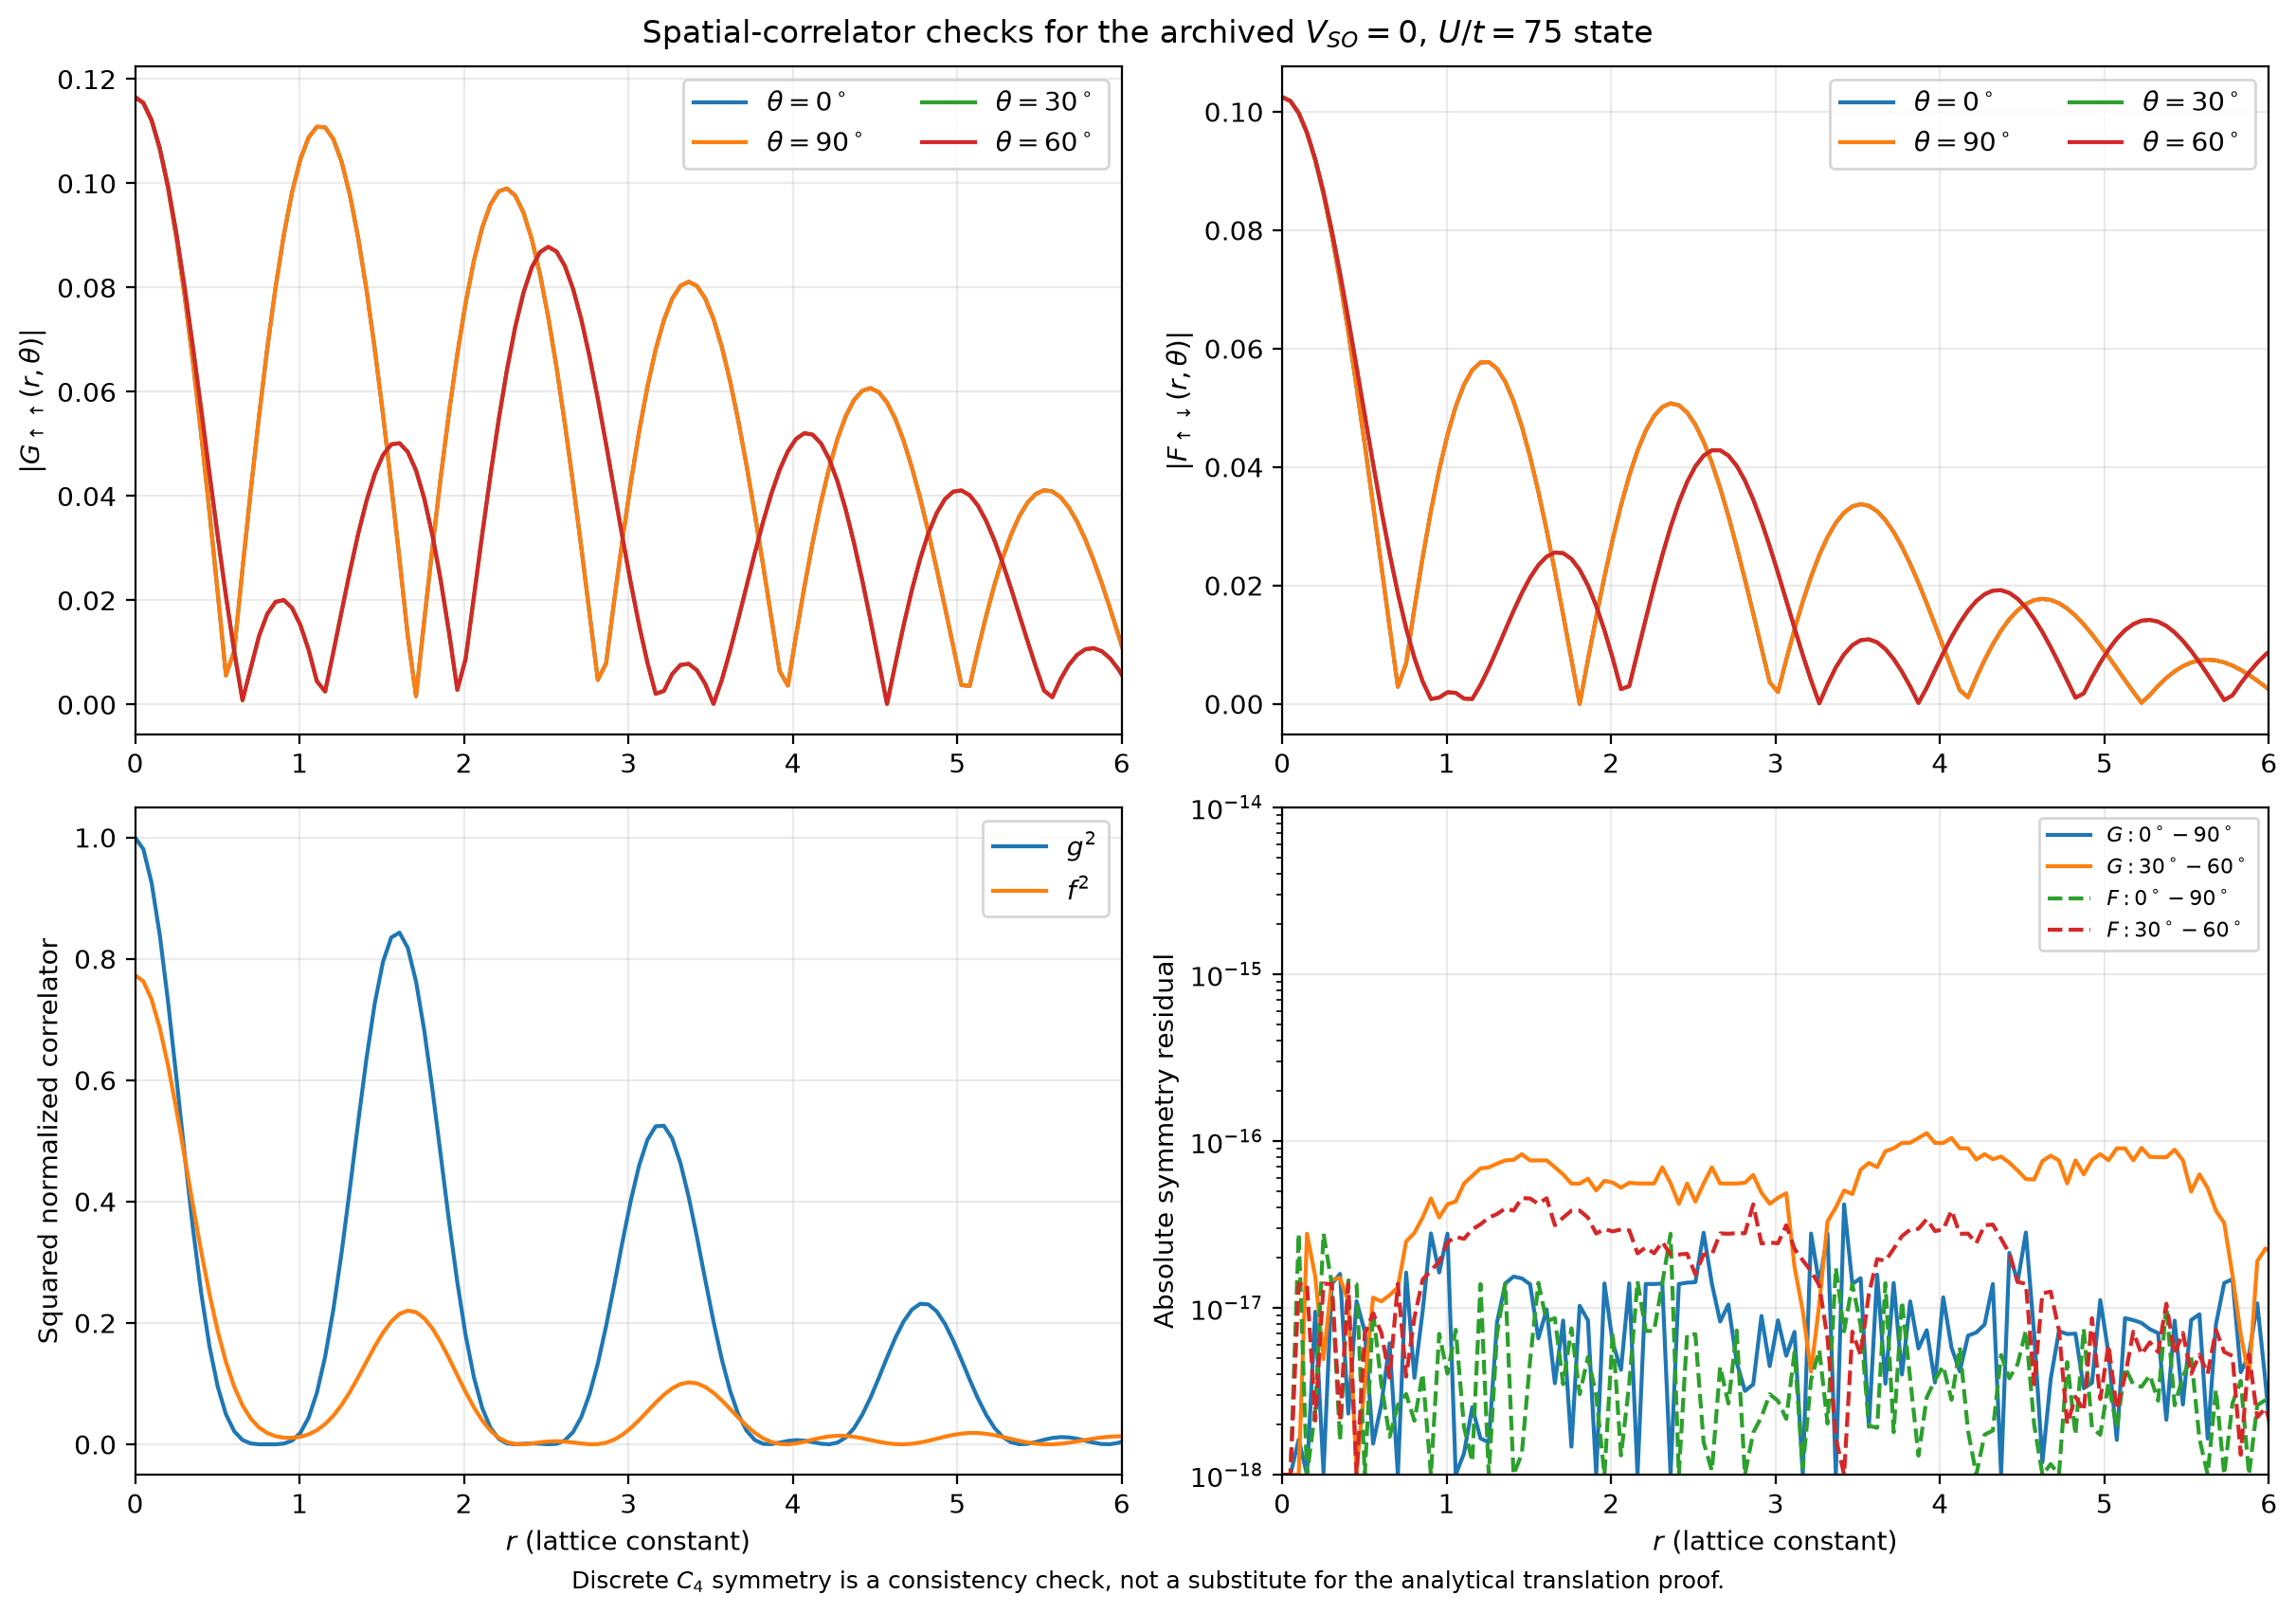
\includegraphics[width=\textwidth]{figs/density_matrix_spatial_checks.png}
\caption{Archived $V_{\SO}=0$, $U/t=75$ normal and anomalous correlators. Directions related by square-lattice symmetry overlap. Maximum residuals are $4.1695\times10^{-17}$ for $G(0^\circ)-G(90^\circ)$, $1.1124\times10^{-16}$ for $G(30^\circ)-G(60^\circ)$, $2.7845\times10^{-17}$ for $F(0^\circ)-F(90^\circ)$, and $4.5431\times10^{-17}$ for $F(30^\circ)-F(60^\circ)$. These are numerical consistency checks, not replacements for the analytical translation proof.}
\label{fig:spatial}
\end{figure}

\subsection{Exact Werner equivalence and positivity}

\begin{figure}[H]
\centering
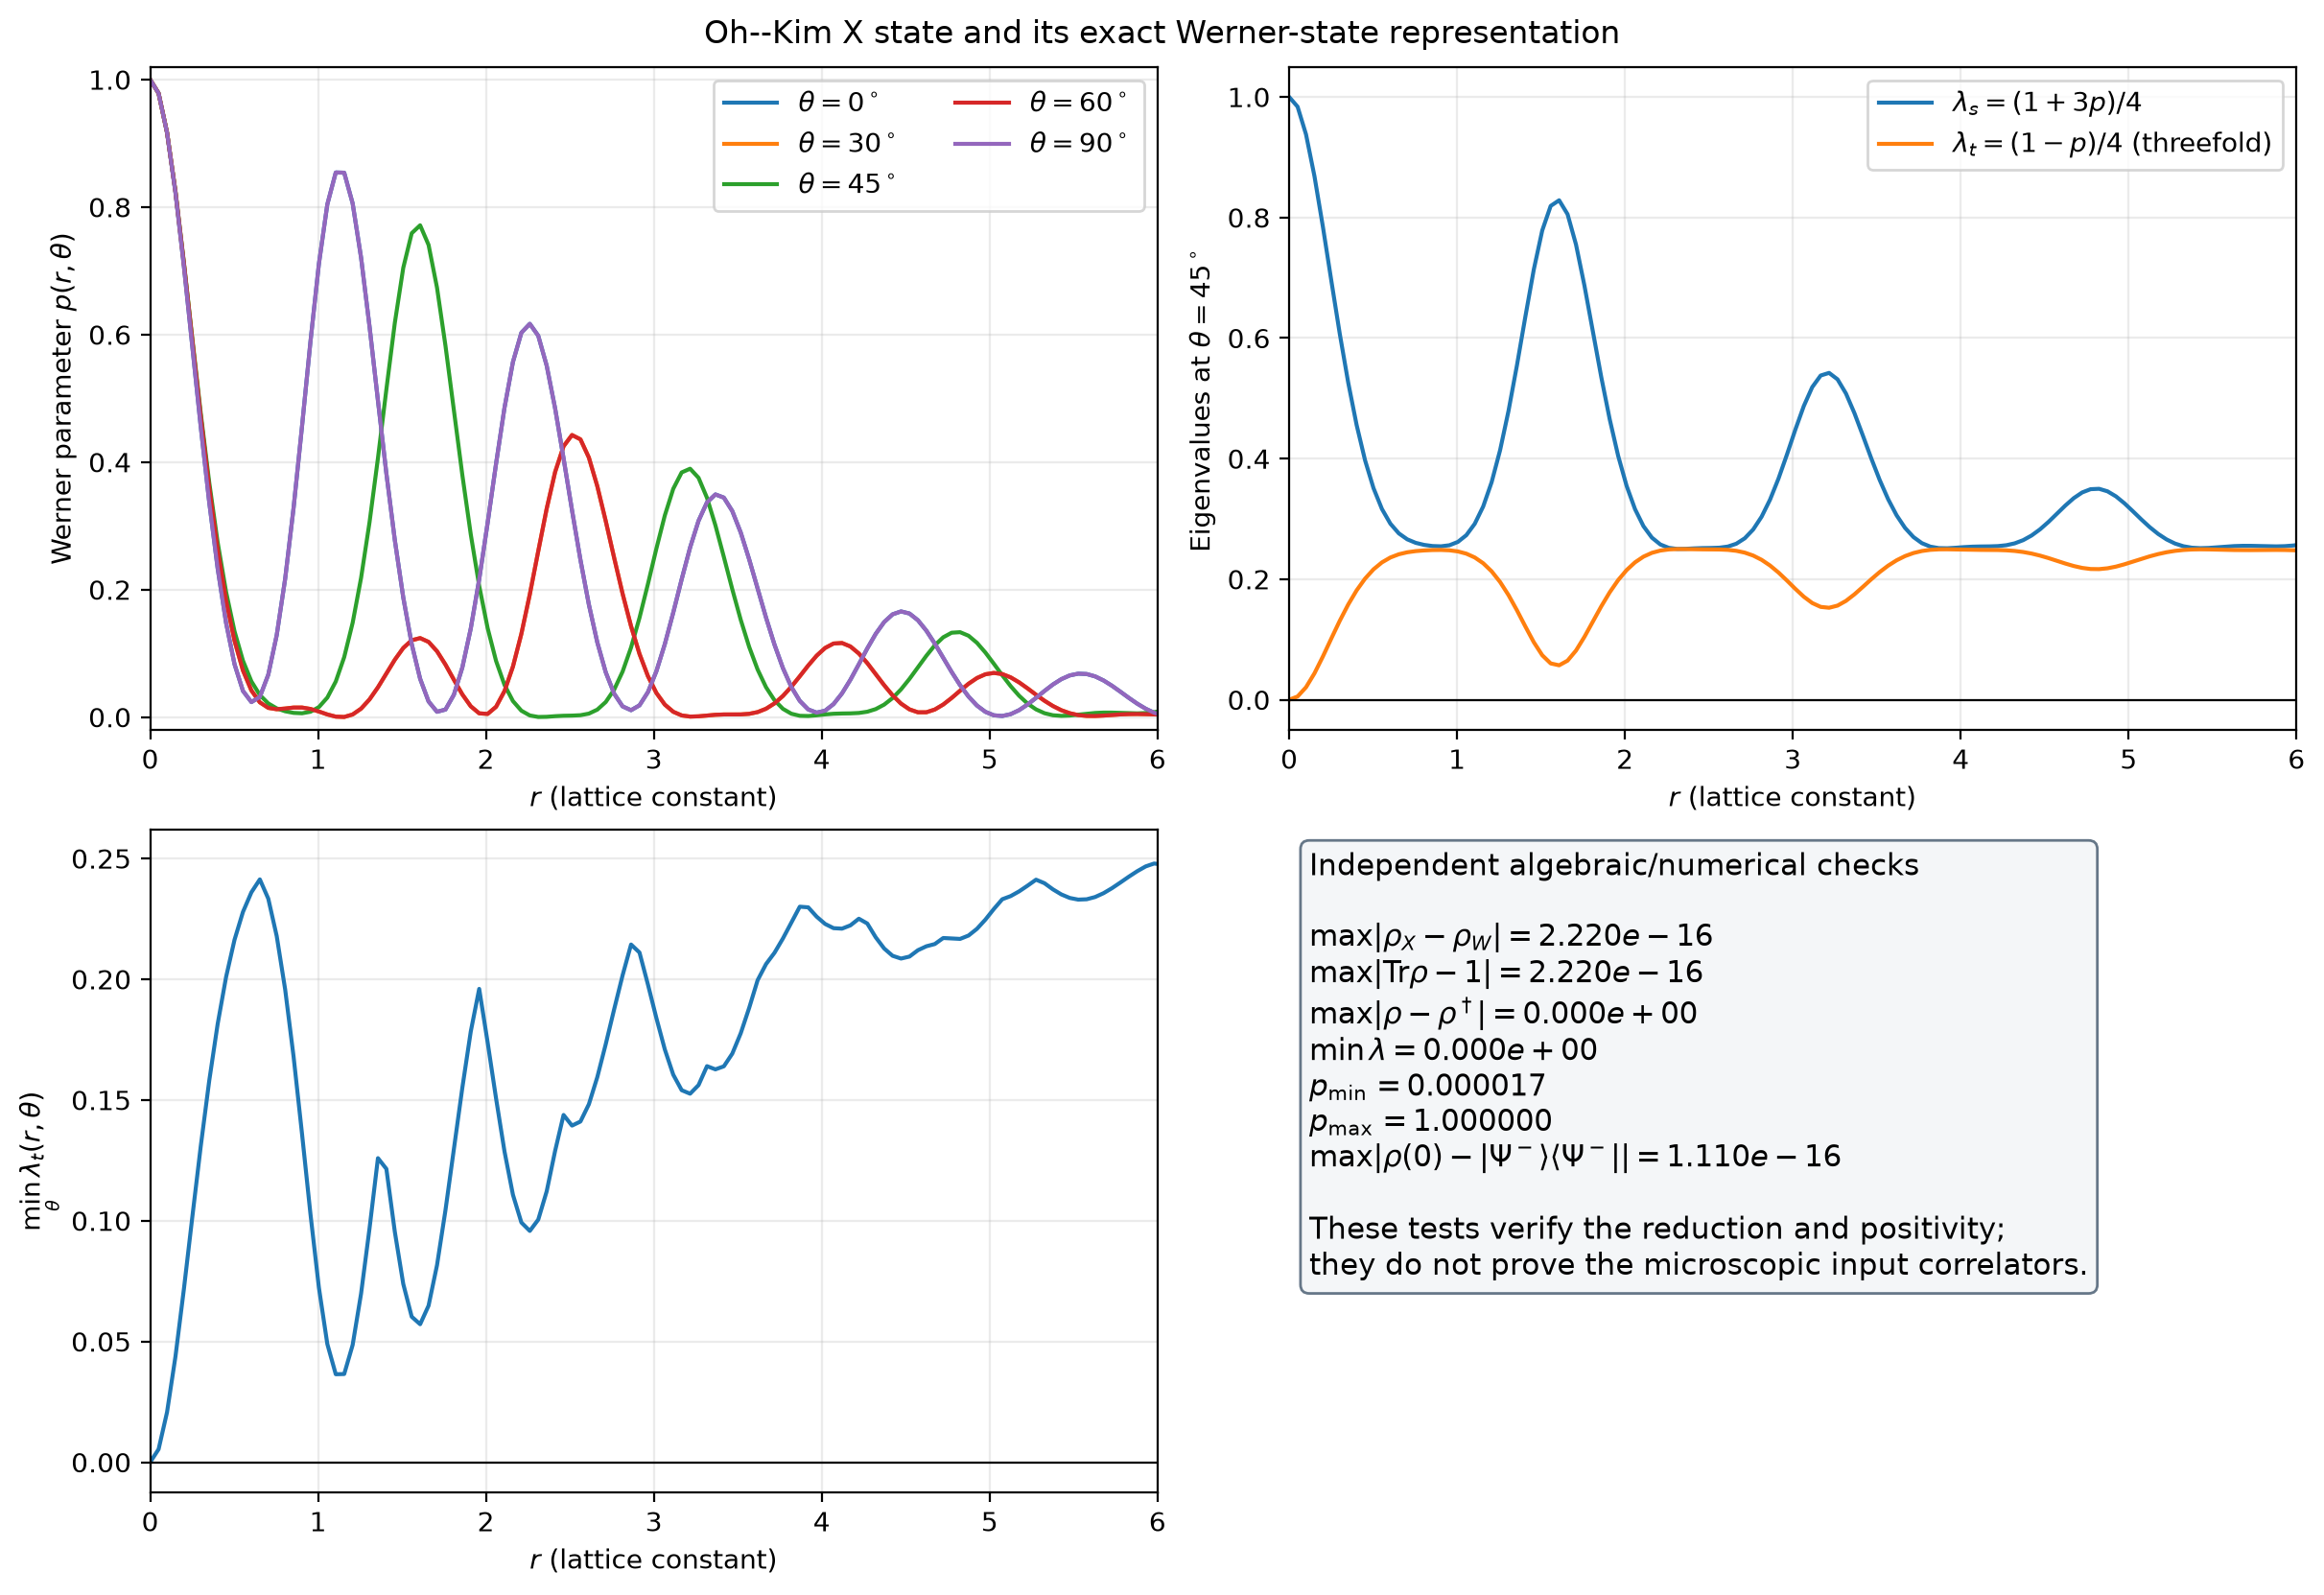
\includegraphics[width=\textwidth]{figs/density_matrix_werner_validation.png}
\caption{Werner parameter and eigenvalues from the archived correlators. Across seven angles and 200 separations, $\max|\rho_X-\rho_W|=2.2204\times10^{-16}$, $\max|\operatorname{Tr}\rho-1|=2.2204\times10^{-16}$, and $\max|\rho-\rho^\dagger|=0$. The minimum eigenvalue is zero at the pure-singlet point, not negative. The range is $1.6806\times10^{-5}\leq p\leq1$, and $\max|\rho(0)-|\Psi^-\rangle\langle\Psi^-||=1.1102\times10^{-16}$.}
\label{fig:werner}
\end{figure}

\subsection{Why the full Rashba case needs a different derivation}
\label{sec:rashba}

Hutchinson \emph{et al.} define
\begin{equation}
c_{\mathbf ks}^{\dagger}=\frac{c_{\mathbf k\uparrow}^{\dagger}+se^{i\theta_{\mathbf k}}c_{\mathbf k\downarrow}^{\dagger}}{\sqrt2}.
\end{equation}
Inverting this relation gives
\begin{equation}
c_{\mathbf k\uparrow}=\frac{c_{\mathbf k+}+c_{\mathbf k-}}{\sqrt2},\qquad
c_{\mathbf k\downarrow}=e^{i\theta_{\mathbf k}}\frac{c_{\mathbf k+}-c_{\mathbf k-}}{\sqrt2}.
\end{equation}
For $n_{\mathbf ks}=\langle c_{\mathbf ks}^{\dagger}c_{\mathbf ks}\rangle$, the original-spin off-diagonal coefficient is
\begin{equation}
\langle c_{\mathbf k\uparrow}^{\dagger}c_{\mathbf k\downarrow}\rangle
=\frac{e^{i\theta_{\mathbf k}}}{2}(n_{\mathbf k+}-n_{\mathbf k-}).
\end{equation}
At $V_{\SO}=0$, degeneracy makes this quantity vanish. At nonzero Rashba coupling it need not vanish.

\begin{figure}[H]
\centering
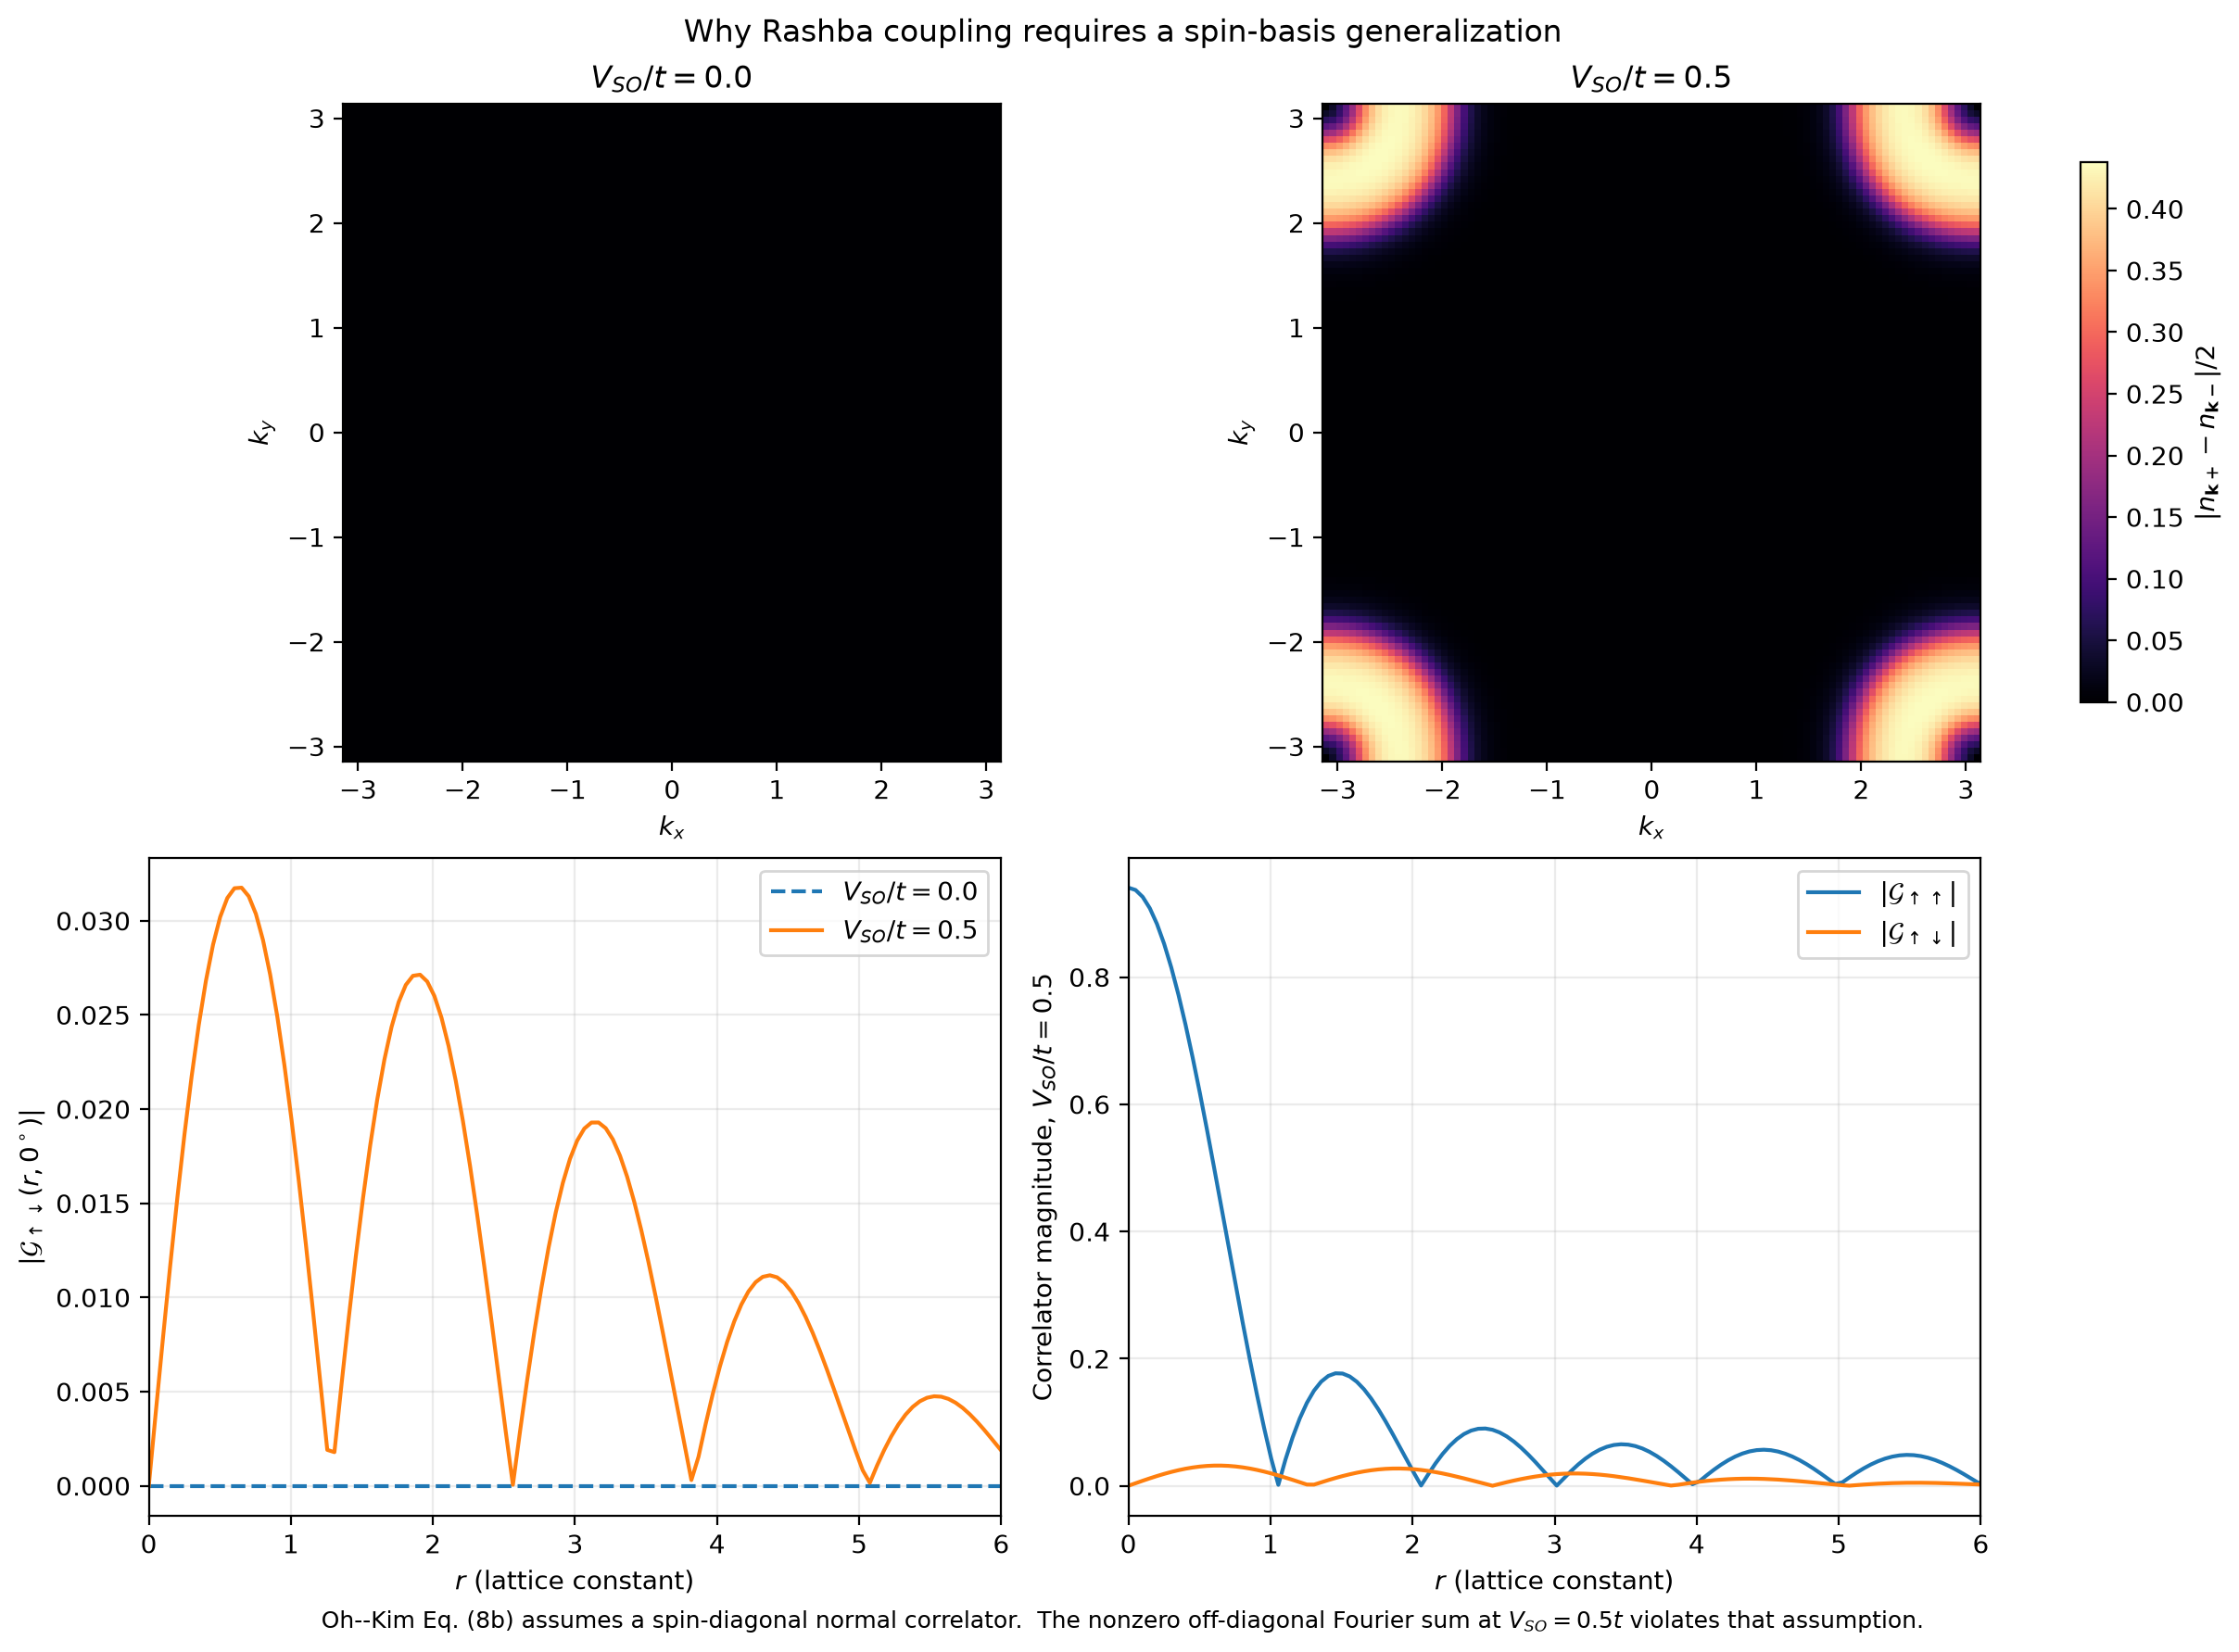
\includegraphics[width=\textwidth]{figs/density_matrix_rashba_scope.png}
\caption{Original-spin normal-correlator diagnostic. The independently executed $V_{\SO}=0.5t$, $U/t=75$ control solution converged with maximum residual $3.526\times10^{-12}$. It gives $\max_r|\mathcal G_{\uparrow\downarrow}(r,0^\circ)|=0.0317533$, whereas the result is exactly zero at $V_{\SO}=0$. This violates Oh--Kim's spin-diagonal assumption in their Eq.~(8b). Translational invariance survives Rashba coupling, but the simple spin reduction does not automatically survive it.}
\label{fig:rashba}
\end{figure}

A nonzero-$V_{\SO}$ treatment must either construct the full spin-resolved $4\times4$ Nambu correlator and derive a generalized two-spin state, or explicitly define helicity pseudospin qubits and justify their different operational meaning.

\section{Separate issue: signed anomalous coherence}
\label{sec:signed}

For the BdG convention stated in the manuscript,
\begin{equation}
u_{\mathbf ks}v_{\mathbf ks}^*=-\frac{\Delta_{\mathbf ks}^*}{2E_{\mathbf ks}}.
\label{eq:signed}
\end{equation}
The archived solver constructs $u_{\mathbf ks}$ and $v_{\mathbf ks}$ as non-negative square roots, and the Green-function routine multiplies those non-negative amplitudes. When $\Delta_{\mathbf ks}$ changes sign, this is not generally equal to Eq.~\eqref{eq:signed} before Brillouin-zone integration.

A separate comparison used the same archived normal $G$, momentum grid, and quadrature, replacing only the anomalous coherence by Eq.~\eqref{eq:signed}.

\begin{figure}[H]
\centering
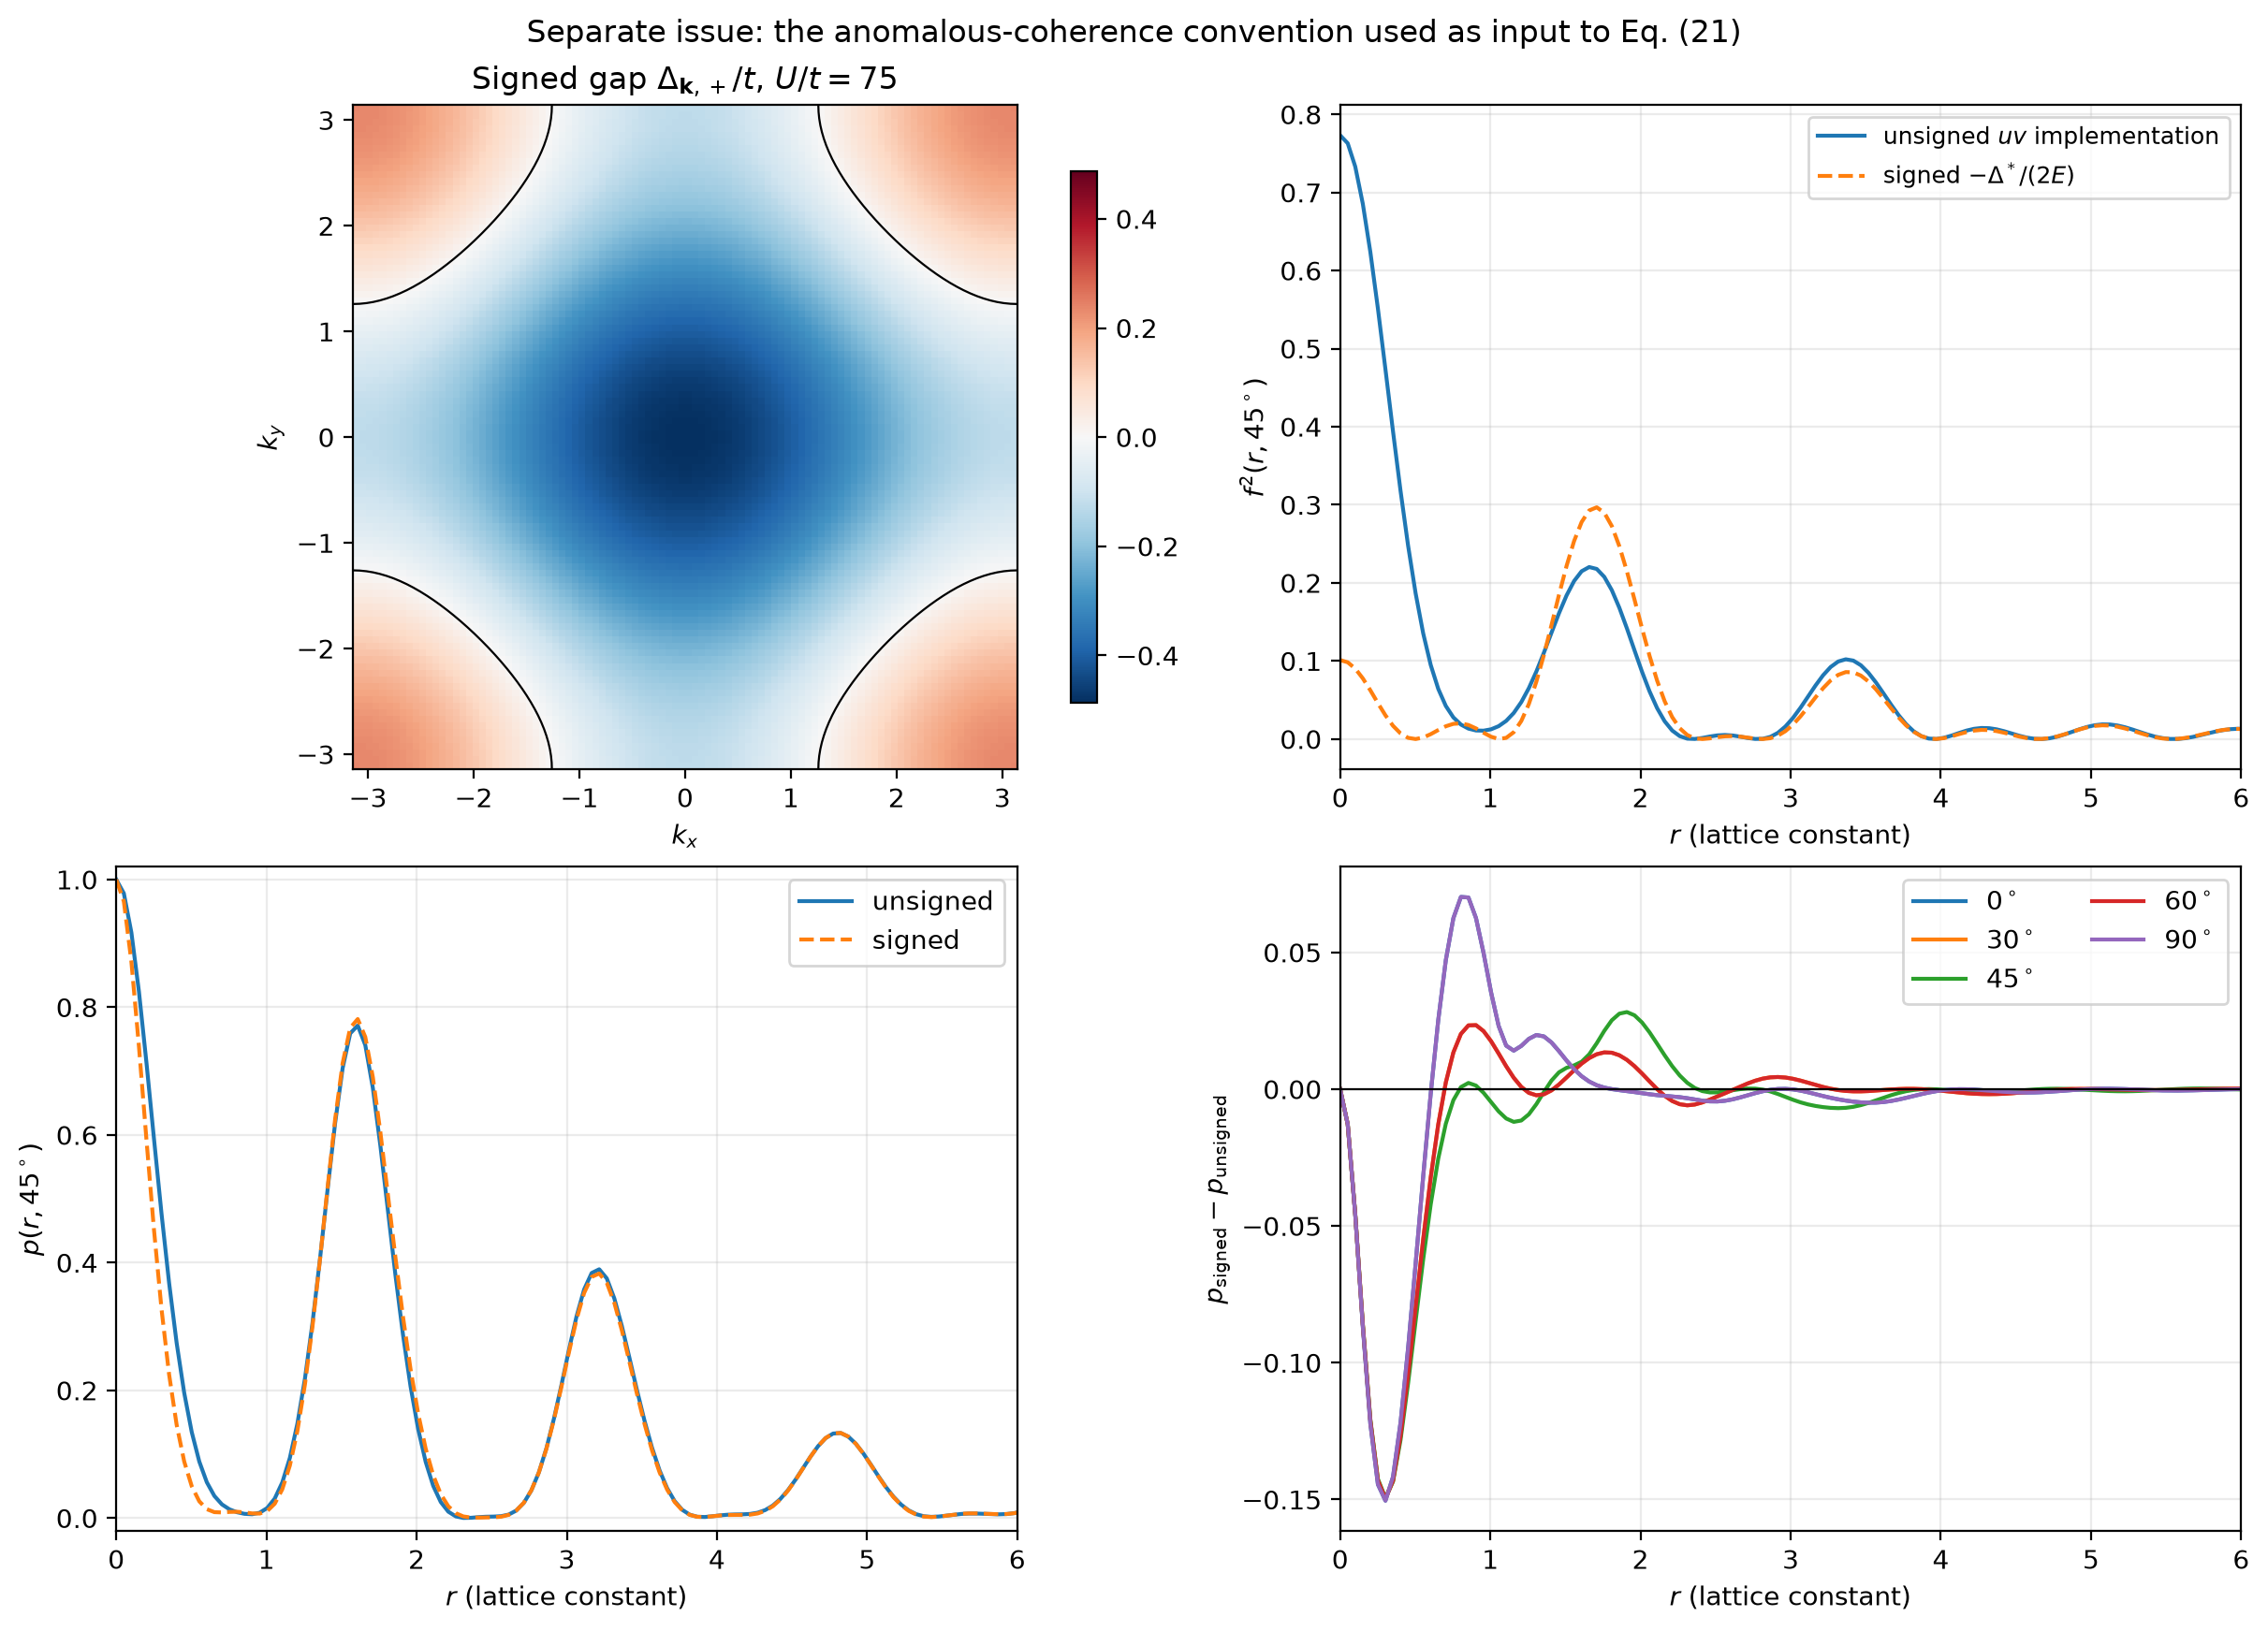
\includegraphics[width=\textwidth]{figs/density_matrix_coherence_convention.png}
\caption{Effect of retaining the gap sign at $U/t=75$, $V_{\SO}=0$. The gap changes sign in the top-left panel. Over the full angular/radial grid, $\max|F_{\mathrm{signed}}-F_{\mathrm{archived}}|=0.1395489$ and $\max|p_{\mathrm{signed}}-p_{\mathrm{unsigned}}|=0.1504256$. The signed-input matrices remain positive and normalized. These are new numerical results and have not been silently substituted into the archived manuscript arrays.}
\label{fig:signed}
\end{figure}

This discrepancy does not invalidate Oh--Kim Eqs.~(19)--(23). It means that the archived numerical values cannot yet be defended as exact signed-BdG results until the anomalous input is corrected or the unsigned approximation is independently justified. The appropriate next step is to regenerate the observables using Eq.~\eqref{eq:signed}, not to change the density-matrix formula.

\section{Scope of the proof}

\subsection*{Established analytically}
\begin{enumerate}
    \item Uniform zero-momentum pairing yields relative-coordinate $G$ and $F$.
    \item Momentum dependence and gap sign changes do not break translational invariance.
    \item Gaussian factorization plus spin-diagonal normal and singlet anomalous correlators yields Oh--Kim Eq.~(19).
    \item The normalized matrix is exactly a Werner state and is positive for $|g|\leq1$.
    \item At $r=0$, it is exactly the singlet.
\end{enumerate}

\subsection*{Established numerically}
\begin{enumerate}
    \item The archived arrays respect square-lattice symmetry to floating-point precision.
    \item The implemented X matrix and independently constructed Werner matrix agree to machine precision.
    \item All tested matrices are Hermitian, normalized, and positive semidefinite.
    \item A nonzero-Rashba control calculation produces original-spin off-diagonal normal correlations.
    \item Retaining the signed gap changes the anomalous input appreciably for the tested $U/t=75$ state.
\end{enumerate}

\subsection*{Not established}
\begin{enumerate}
    \item Applicability of the unchanged matrix to original-spin qubits at $V_{\SO}\neq0$.
    \item Exactness beyond Gaussian BdG mean-field theory.
    \item Applicability to open boundaries, impurities, position-dependent pairing, or finite-momentum pairing.
    \item Correctness of the archived unsigned anomalous correlator as an exact signed-BdG result.
    \item A canonical fixed-electron-number reduction beyond the conditional two-detection normalization used by Oh and Kim.
\end{enumerate}

\section{Manuscript-ready justification}

\begin{quote}
In the zero-spin-orbit-coupling limit considered in the numerical calculations, the two helicity branches are degenerate and the original spin basis is restored. The spatially uniform BdG mean-field Hamiltonian contains only zero-center-of-mass-momentum pairs, so the equal-time normal and anomalous correlators depend on the relative coordinate $\mathbf r=\mathbf R_1-\mathbf R_2$. Because the BdG state is Gaussian, its two-particle contraction factorizes by Wick's theorem. The normal correlator is spin diagonal and the even-parity anomalous correlator has singlet spin structure. Conditioning on one electron detected at each position and normalizing the resulting two-spin sector therefore yields the Oh--Kim matrix, Eqs.~(19)--(23) of Ref.~\cite{OhKim}, including for the momentum-dependent extended-$s$-wave gap. This reduction is not used for original-spin qubits at nonzero Rashba coupling, where spin-off-diagonal normal correlations and mixed singlet--triplet pairing require a generalized spin-resolved construction. The anomalous spatial input is evaluated using the signed BdG coherence factor $u_{\mathbf k}v_{\mathbf k}^*=-\Delta_{\mathbf k}^*/(2E_{\mathbf k})$.
\end{quote}

The final sentence should be included only after the numerical pipeline actually uses the signed factor.

\section{Reproducibility}

Run from the repository root:
\begin{center}
\texttt{.venv/bin/python analysis/validate\_density\_matrix\_scope.py}
\end{center}
The script generates \texttt{reports/density\_matrix\_validity\_checks.json}, \texttt{data/density\_matrix\_validity\_checks.npz}, and the four figures in \texttt{figs/}. No IBM hardware or external numerical results were used. The nonzero-Rashba example is a newly executed control calculation, not part of the archived manuscript sweep.

\begin{thebibliography}{9}
\bibitem{OhKim}
S. Oh and J. Kim, \emph{Entanglement of electron spins in superconductors}, Phys. Rev. B \textbf{71}, 144523 (2005), \url{https://arxiv.org/pdf/quant-ph/0406013}.

\bibitem{Hutchinson}
J. Hutchinson, J. E. Hirsch, and F. Marsiglio, \emph{Enhancement of superconducting $T_c$ due to the spin-orbit interaction}, \url{https://arxiv.org/pdf/1801.08988}.
\end{thebibliography}

\end{document}
